\section{Motivation and problem}
\label{sec:background}


\begin{figure*}
\centering
\subfloat[\Process~$R$ efficiently advertises its content using epidemic propagation. Every \process requests $R$ if needed.\label{fig:partition_intuitionA}]{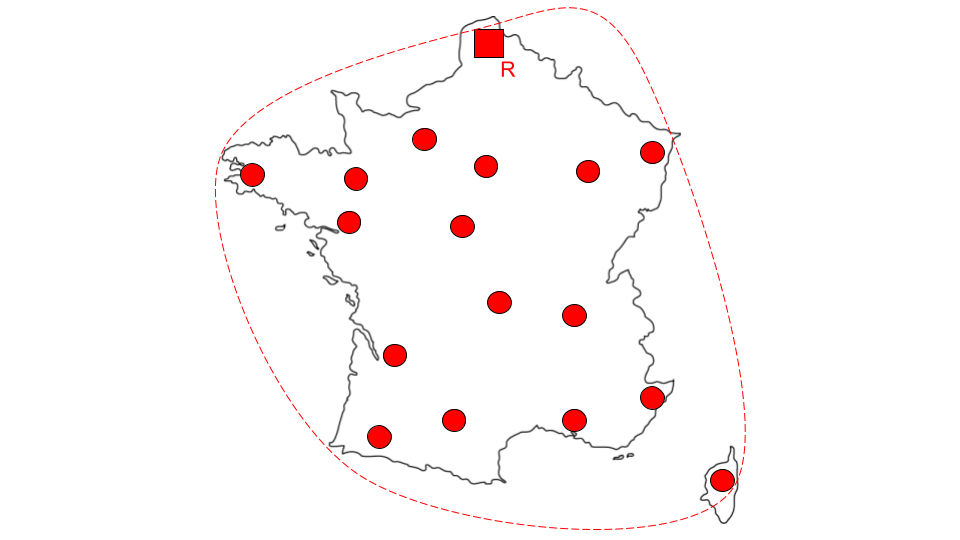
\includegraphics[trim=6cm 0.33cm 6cm 0.33cm, clip, width=0.24\textwidth]{img/Dynamic-partitioning-1.png}}
\hfill
\subfloat[\Process $G$ creates a second replica splitting the red set in two. \Processes request their closest replica host.\label{fig:partition_intuitionB}]{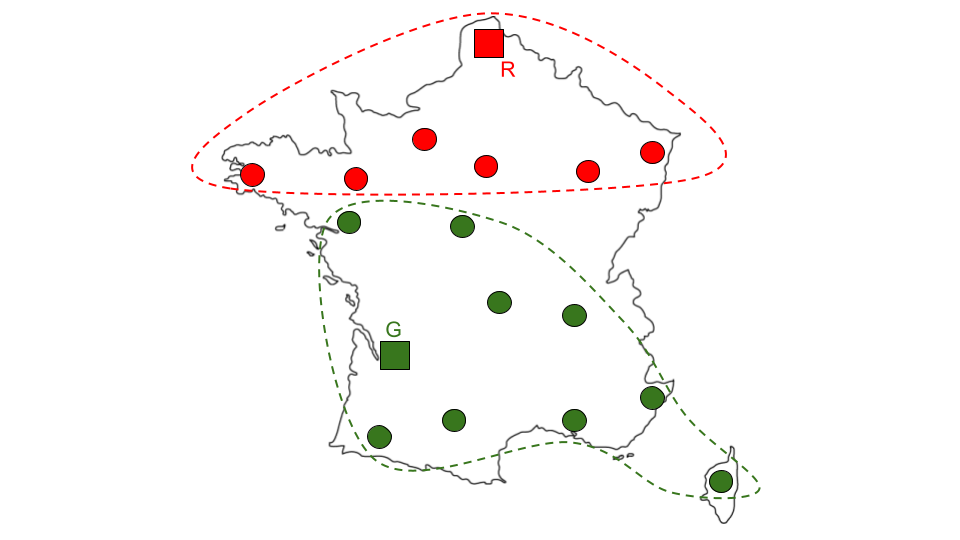
\includegraphics[trim=6cm 0.33cm 6cm 0.33cm, clip, width=0.24\textwidth]{img/Dynamic-partitioning-2.png}}\hfill
\subfloat[\Process $B$ creates another replica. \Process~$B$ needs to notify only a small subset of \processes.\label{fig:partition_intuitionC}]{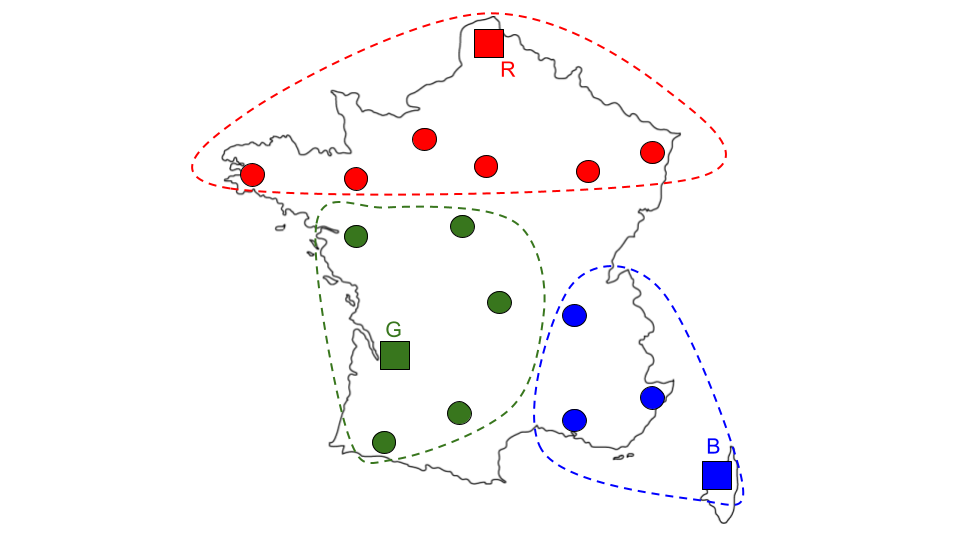
\includegraphics[trim=6cm 0.33cm 6cm 0.33cm, clip, width=0.24\textwidth]{img/Dynamic-partitioning-3.png}}\hfill
\subfloat[\Process $G$ destroys its replica. \Processes that belong to its partition must find the closest partition they are in.\label{fig:partition_intuitionD}]{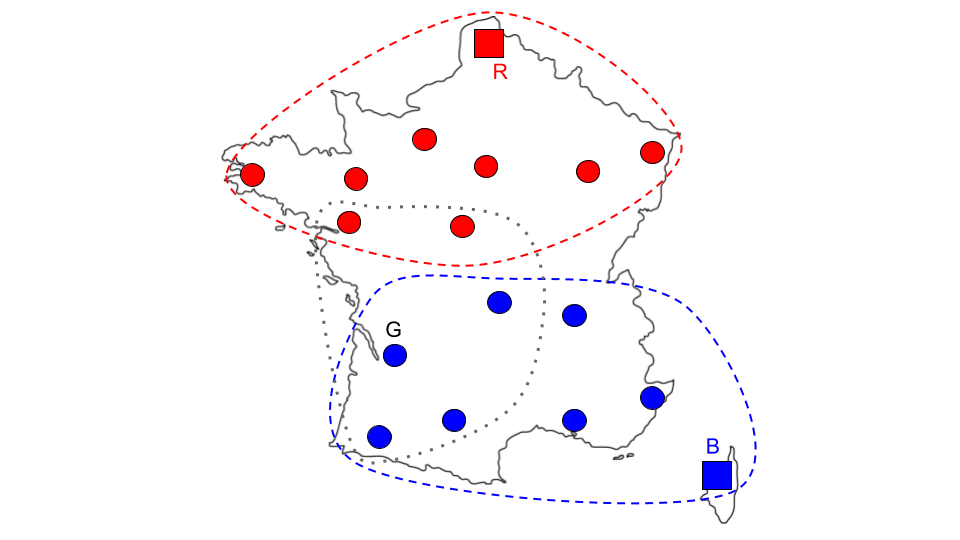
\includegraphics[trim=6cm 0.33cm 6cm 0.33cm, clip, width=0.24\textwidth]{img/Dynamic-partitioning-4.png}}
%
\caption{The french RENATER topology. Partitions
  grow and shrink depending on creations and removals of
  replicas.} \label{fig:partition_intuition}
\end{figure*}

%%% Local Variables: 
%%% mode: latex
%%% TeX-master: "../paper"
%%% ispell-local-dictionary: "english"
%%% End: 
 %% positioning

Numerous studies addressed content indexing in geo-distributed
infrastructures ranging from centralized services to fully
decentralized approaches~\cite{squirrel}. We advocate for the latter
where \processes host the service themselves so they do not need to
request remote -- possibly far away third-party -- entities to
retrieve content locations.  More precisely, we propose to consider the content
indexing issue as a dynamic logical partitioning problem. This section
motivates our positioning and explains the shortcomings of existing
implementations.

%% Numerous studies exist on content indexing, with solutions being
%% either centralized or distributed (see
%% Section\ref{related_work}). As explained above, in this paper we
%% advocate designs that do not rely on requesting any remote entity
%% before being able to access a given content.  This section thus
%% focuses on the existing solutions so that: \textbf{for any content,
%% every node is able to access its closest replica without any prior
%% request.}  We explain why existing implementations are costly thus
%% preventing their deployment in real systems.  Then, we describe the
%% problem tackled by this paper at an abstract level to underline the
%% challenges that drove the design of our proposal.

\begin{asparadesc}
\item [Dissemination:]

Figure~\ref{fig:partition_intuition} depicts an infrastructure
comprising 17 interconnected \processes spread across France. In
Figure~\ref{fig:partition_intuitionA}, a single \Process~$R$ hosts the
content, so every other \process downloads from this \process when it
needs it. In that regard, \Process~$R$ only needs to disseminate a
message notifying all other \processes of its new
content. \Process~$R$ can use uniform reliable
broadcast~\cite{hadzilacos1994modular} and epidemic
propagation~\cite{epidemic-protocol} to guarantee that every \process
eventually knows the content location by efficiently using
neighbor-to-neighbor communication.

\item [Location:]

Then, in Figure~\ref{fig:partition_intuitionB}, another \Process~$G$
creates a replica of this content. Similarly to \Process~$R$, it
notifies other \processes of this new replica. However, to avoid that
north \processes request its replica, and south \processes request the
northern one, \processes hosting a replica must add \emph{location
information} along with their notifications. As a consequence, every
\process eventually knows every replica location and can download from
its closest host. \underline{R}ed \processes would request
\Process~$R$ while \underline{g}reen \processes would request
\Process~$G$.

\item [Scoped broadcast:]

Then, in Figure~\ref{fig:partition_intuitionC}, another \Process~$B$
creates a replica of this content. Similarly to \Process~$R$ and
\Process~$G$, \Process~$B$ can notify other \processes of this new
replica. However, the set of \processes that could actually use this
new replica is actually much smaller than the network size. Uniform
reliable broadcast is not designed for such a context and would
generate a lot of unnecessary traffic. Instead, \processes need a
communication primitive that propagates notifications within a scope
by evaluating a predicate, starting at its broadcaster (the
\emph{source}).  In other terms, \processes propagate notifications as
long as they consider them useful based on location information they
carry. We call such a primitive \emph{scoped broadcast} (see
Section~\ref{subsec:scoped}), for messages transitively reach a subset
of interconnected \processes (the \emph{scope}). Using this primitive,
\processes can lock down the traffic of content indexing to relevant
\processes.

\item [Logical partitioning:]

Every \process ends up with at least one known replica that is its
closest. The set of interconnected \processes with the same closest
replica is a \emph{partition}. Every \process belongs to one, and only
one, partition (see Section~\ref{subsec:consistent}).
In Figure~\ref{fig:partition_intuitionC}, there are three logical partitions.

%% Contrarily to membership
%% protocols that choose neighboring \processes to communicate with based
%% on metrics~\cite{t-man}, \processes in our context have no control
%% over their neighboring \processes: they cannot add nor remove
%% communication links.

\item [Dynamic partitioning:]

In Figure~\ref{fig:partition_intuitionD}, \Process $G$ destroys its
replica. Every \process that belonged to its green partition must
choose another partition to be in. While it makes sense for
\Process~$G$ to scoped broadcast its removal, \Process~$B$ and
\Process~$R$ cannot afford to continuously advertise their replica to
fill the gap left open by \Process~$G$. A better approach would
consist in triggering scoped broadcast at bordering \processes of red
and blue partitions once again. In other words, the scope of scoped broadcast changes
over receipts by \processes. This dynamic partitioning raises additional
challenges related to concurrent operations where removed partitions
could block the propagation of other partitions (see
Section~\ref{subsec:dynamic}).
%% \item [Lazy partitioning:]
%% \TODO{Finally, in Figure~\ref{fig:partition_intuition}, every nodes of
%%   the system maintains an index to every content. In systems
%%   comprising billions of content, this could constitute a scalability
%%   issue. The partitioning protocol should take advantage of boundary
%%   between autonomous systems in the Internet. For instance, the AS
%%   from France should not flood the AS from Spain unless the latter
%%   starts to host a replica. In addition, when the system removes its
%%   last source, it should stop receiving messages from other ASes
%%   designed to maintain the closest partition.}
Next Section details the properties of scoped broadcast and dynamic
partitioning, % in dynamic networks,
and provides an implementation called \NAME.% along with its complexity.
\end{asparadesc}

%% \subsection*{Disseminate localization information}
%% Enabling the accessibility of content without prior requests implies
%% that the information about replica localization has to be pushed
%% directly to the nodes.  Broadcasting information about cache updates
%% to all nodes in the system is a straightforward way to maintain
%% consistent information about replica localization for all
%% nodes~\cite{nlsr,lscr}. Indeed, having the entire knowledge of all the
%% replica localizations along with distance information carried into
%% messages, each node can easily compute where the closest copy of a
%% given object resides, without contacting any remote node. Moreover,
%% removing the lookup latency directly involves faster downloading
%% times.  Similarly, one could solve this issue by using a conflict-free
%% replicated datatype (CRDT) for set data structures, for
%% example~\cite{shapiro2011crdts}.  However, either by broadcasting or
%% with CRDTs, both inherently imply that every nodes will eventually
%% receive all messages.  That means information that might only
%% interests a small subset of nodes is actually spread out all over the
%% network.

%% \subsection*{Locking down the dissemination}
%% To provide the intuition underlying our proposal, we now describe the
%% problem tackled by this paper at an abstract level, and explain how an
%% (imaginary) omniscient entity could solve it.  In this way, suppose
%% there exists an \textit{oracle} in the system that instantly knows the
%% arrival/departure of nodes in the topology and the location of the
%% creation/removal of replicas. In other words, this oracle is
%% constantly aware of the current topology and the current list of all
%% available replicas of a given content in the system. Equipped with
%% these two information, it is then trivial for this oracle to compute
%% for each node, where resides its closest replica for a given
%% content. Mapping each node of the topology to a single replica amounts
%% to partition the set of all nodes into $k$ disjoint sets (or
%% partitions), where $k$ is the number of current replicas. Thus, every
%% node in the same partition would get the content from the same
%% replica. Interestingly, this partitioning matches the physical
%% topology as neighbors physically closed in the infrastructure will
%% most likely reside in the same partition.  For any event such as an
%% arrival/departure of nodes or creation/removal of replicas, the oracle
%% is thus able to inform the \textit{exact} subset of nodes that has to
%% update their location (\ie the exact scope of an event).


%% This is illustrated in Figure~\ref{fig:partition_intuition} where we
%% depict the partitions shrinking or expanding according to the creation
%% or removal of replicas respectively.  In Figure\ref{fig:1a}, there
%% exists a single occurence of a given content in node $R$: all nodes
%% thus belong to the same partition as they would all retrieve the
%% content from the same node.  A second replica is created in node $G$
%% in Figure~\ref{fig:1b}, resulting in $2$ partitions. Nodes from the
%% \textit{green} partition would all obtain the content from node $G$ as
%% it is their closest replica, while nodes from the \textit{red}
%% partition would get it from node $R$.  Note that only the nodes in the
%% green partition has to be informed of the creation of the replica in
%% node $G$. Similarly, in Figure~\ref{fig:1c}, only nodes in the blue
%% partition should be informed of the creation of a new replica in node
%% $B$ as it does not impact other nodes.  Finally, when the replica in
%% node $G$ is removed, nodes in the stale green partition have to join
%% existing ones as illustrated in Figure~\ref{fig:1d}.  The challenge of
%% implementing such a partitioning in an asynchronous network resides in
%% informing this minimal subset of nodes (or as close as possible),
%% without any \textit{a priori} knowledge while only relying on local
%% information (\ie no node has the knowledge of all the replica
%% localizations).


%% Finally, we emphasize that information about a given replica
%% localization should remain in a given geographical scope.
%% Intuitively, it is most likely that events happening at a given place
%% in the network will have no impact on nodes that are very far away
%% from them.  This prevents the use of gossip protocols for example.
%% Indeed, gossip protocols are also appealing candidates to disseminate
%% information reliably across a network~\cite{epidemic-protocol} and
%% numerous studies have shown how quickly they converge despite high
%% level of churn and/or failures~\cite{lpbcast}.  However, these
%% protocols usually relies on a so-called \textit{peer-sampling
%%   service}~\cite{jelasity2007gossip} to efficiently propagate the
%% information. This implies that nodes will exchange messages with
%% random nodes in the system far exceeding their geograhical scope.


%%% Local Variables: 
%%% mode: latex
%%% TeX-master: "../paper"
%%% ispell-local-dictionary: "english"
%%% End: 
